% !TeX spellcheck = fr-moderne
\section{Introduction de l'industrie de la télécommunication}
\subsection{L'evolution des normes de téléphonie mobile}
Depuis 1984, il y a déjà plusieurs standards ont été utilisé par les opérateur dans le monde entier. Voici un tableau de différentes standards mobile en Europe et ses paramétrés \ref{tbl:GMIE}. 
\begin{table}[H]
\begin{tabular}{|p{2cm}|p{2cm}|p{2cm}|p{4cm}|}
	\hline
	Génération&Acronyme&Description&Débit\\
	\hline
	1G		&Radiocom 2000	&Échanges de type voix uniquement&analogique\\
	\hline
	\hline
	2G		&GSM			&Échanges de type voix uniquement	&9,05 kbps\\
	\hline
	2,5G	&GPRS			&Échange de données sauf voix		&171,2 kbps / 50 kbps / 17,9 kbps\\
	\hline
	\hline
	3G		&UMTS			&Voix + données						&144 kbps rurale, 384 kbps urbaine, 1,9 Mbps point fixe / -\\
	\hline
	3.5G ou 3G+ ou H&HSPA	&Évolution de l'UMTS				&14,4 Mbps / 3,6 Mbps / -\\
	\hline
	\hline
	4G		&LTE			&Long Term Evolution (Données)				&150 Mbps / 40 Mbps / -\\
	\hline
	4G		&LTE-Advanced	&Long Term Evolution Advanced (Données+voix)		&1 Gbps à l'arrêt, 100 Mbps en mouvement / - / -\\
	\hline
\end{tabular}
\caption{Les différentes générations de téléphonie mobile en Europe}
 \label{tbl:GMIE}
\end{table}

\subsubsection{La premier génération}
En télécommunication, \textsf{1G} est la premier génération des standards pour la téléphonie mobile, il s'agit de la première apparition du réseaux de téléphonie mobile, 1G sont des réseaux analogiques, peut échanges de type voix uniquement.
\subsubsection{La deuxième génération}
\textsf{2G}, la technologie de téléphonie sans fil de deuxième génération, la différence entre le réseaux 1G et 2G est: le signaux radio sur les réseaux 1G sont analogiques, et celle de 2G sont numériques.

Systèmes 2G ont été significativement plus efficaces du spectre permettant de bien plus grand taux de pénétration du téléphone mobile, en plus les données vocales numériques peuvent être compressées et multiplexées beaucoup plus efficacement que les codages de la voix analogique grâce à l'utilisation de codecs différents, ce qui permet plus d'appels à transmettre dans la même quantité de bande passante radio. Et 2G présenté premier foi les services de données pour mobile. Les Technologie 2G permettent les divers réseaux de téléphonie mobile de utiliser des services tels que le SMS et MMS. Tous les message de texte envoyés au delà de 2G sont chiffrés numériquement, ce qui permet le transfert de données de telle sorte que seul le destinataire peut recevoir et lire.   

Réseaux 2G ont été construits principalement pour les services téléphoniques et de transmission de données lent (défini dans les documents de spécifications IMT-2000).

Réseaux \textsf{2,5G}, on le qualifie souvent de le General packet Radio Service ou GPRS, est une norme pour la téléphonie mobile dérivée du GSM et complémentaire de celui-ci, permettant un débit de données plus élevé. Le 2,5 indique que c'est une technologie à mi-chemin entre le GSM (deuxième génération) et l'UMTS (troisième génération). Le GPRS est une extension du protocole GSM : il ajoute par rapport à ce dernier la transmission par paquets. Cette méthode est plus adaptée à la transmission des données. En effet, les ressources ne sont allouées que lorsque des données sont échangées, contrairement au mode « circuit » en GSM où un circuit est établi – et les ressources associées – pour toute la durée de la communication. Le GPRS a ensuite évolué au début des années 2000 vers la norme \textsc{edge} également optimisée pour transférer des données et qui utilise les mêmes antennes et les mêmes fréquences radio.
\subsubsection{La troisième génération}
La troisième génération (3G) des normes de téléphonie mobile. Elle est représentée principalement par W-CDMAmm, CDMA2000, TD-SCDMA et WiMAX. Elle permettant des débits de 2 à 42 Mb/s qui sont bien plus rapides qu'avec la génération précédente. Grâce à l'utilisation des règles de classement de l'utilisateur, et les  bandes de fréquences supérieures rendant la capacité du réseau augmenter.

Dans les différentes standard  3G et ses prédécesseur, ils utilisent le domaine CS (Circuit Switch)  pour les services vocaux, et le domaine PS (Packet Switch) s'occupe des services de données \ref{Fig.3G.1}.
\subsubsection{La quatrième génération}
La quatrième génération des standards pour la téléphonie mobile, succédant à la 2G et la 3G, en théorie, elle permet de transmette de données à des débits supérieur à 100 Mb/s. 

Une des particularité de la 4G est sa EPC (Evolved Packet Core) est basé sur IP, et il n'y a plus de mode commuté (le 'Circuit Switched Domain' qui s'occupe le service vocaux dans les standard précédant), ce qui signifie que les services vocaux transmis sur l'internet \ref{Fig.3G.2}. 



\begin{figure}[H]
	\centering
	\subfigure[Réseau 3G et ses prédécesseur]{
		\label{Fig.3G.1}
		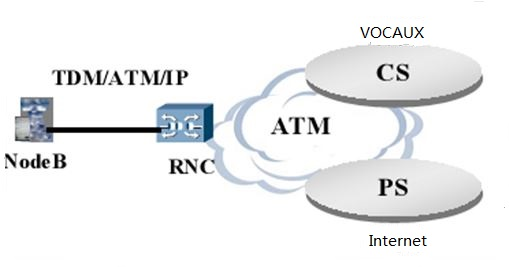
\includegraphics[width=3in]{images/3G2.JPG}}\hfill		
	\hspace{1in}
%\flushright
	\subfigure[Réseau 4G]{
		\label{Fig.3G.2}
		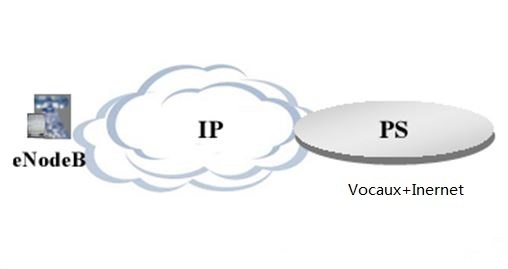
\includegraphics[width=3in]{images/4g.JPG}}
	\caption{Structure des réseaux} 
		\label{Fig.3G}
\end{figure}
Les avantages du réseau 4G sont:  plus haut débit, mieux utilisation de la bandes de fréquence, moins de délai (délai dans le panneau de l'utilisateur est inférieur que 5 ms, délai dans le panneau de commande est inférieur que 100 ms ), plus simple structure du réseau, moins de consommation d'énergie Terminal.

\subsection{Le réseau LTE}
Le LTE (Long Term Evolution) est l'evolution la plus récent des normes de CDMA 2000, TD-SCDMA, GSM. La norme LTE. La technologie LTE été considérée comme une norme de troisième génération '3.9G', et la 'vraie 4G', appelée LTE-Advanced été reconnu par l'UIT comme une technologie 4G en 2010. LTE a deux branche: LTE-FDD (Frequency-Division Duplex  Long Term Evolution)et LTE-TDD, (Time Division Duplex Long Term Evolution)les deux standards sont similaire, la différence entre les deux standard est moins de 15\% \ref{evolution}. En 2011-2012, les réseaux LTE-TDD sont commercialisés sous l'appellation 4G par CMCC un Chine.
      \begin{figure}[H]
          \centering
          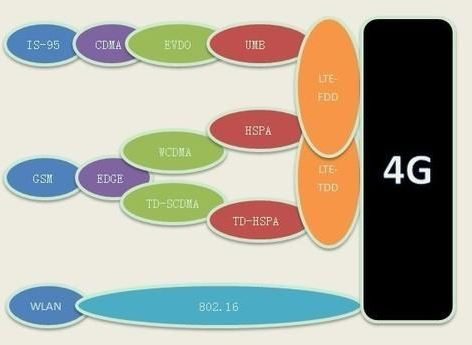
\includegraphics[width=4in]{images/evolution.JPG}
          \caption{l'evolution des standard}
          \label{evolution}
      \end{figure}
      
\subsubsection{La structure du réseau LTE}
Le réseau 4G contient 3 partie: UE( User Equipment);, eNodeB (les stations de base), EPC (Evolved Packet Core). EPC contient MME, S-GW, P-GW et HSS \ref{structure4G}  \ref{founction du chaque partie}. 
    
      \begin{figure}[H]
          \centering
          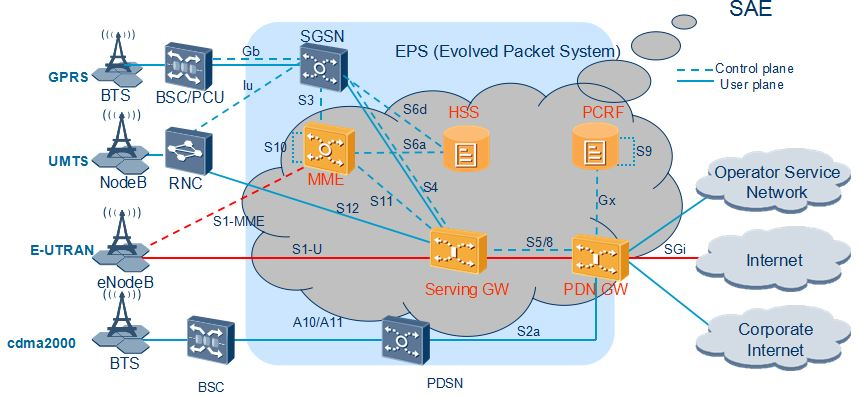
\includegraphics[width=5in]{images/enb2.jpg}
          \caption{la structure du réseau}
          \label{structure4G}
      \end{figure}
      
\begin{table}[H]
	\begin{tabular}{|>{\centering\arraybackslash}p{2cm}|>{\centering\arraybackslash}p{11 cm}|}
		\hline Part &                     Fonction\\
		\hline MME & 
			L'authentification des utilisateurs et la gestion des clés,  Cryptage de la couche NAS,  Gestion de la liste TA, Sélection P-GW ou S-GW \\ 
		\hline Service Gateway & Compression d'en-tête IP, Routage de paquets et la transmission, La commutation entre eNB, Facturation des utilisateurs porteur \\ 
		\hline PDN Gateway & L'allocation des adresses IP de UE, l'accès aux fonction de gestion de réseau externes, Facturation en service \\ 
		\hline HSS(Home Subscriber Service) & Stockée données de l'utilisateur associées au service \\ 
		\hline PCRF & Roaming \\ 
		\hline 
	\end{tabular} 
	\caption{la fonction du chaque partie}
	\label{founction du chaque partie}
\end{table}    

Entre deux \textsc{e-utran}, il y a l'interface X2, l'interface S-11 se trouve entre S-GW et MME, \textsc{e-utran} et S-GW échange les données par l'interface S1-U \ref{Fig.S1}et il échange les donnée par l'interface S1-AP avec MME \ref{Fig.S1}, MME et HSS utilise l'interface S6A, et l'interface S5/8 entre S-GW et P-GW, Gx entre PCRF et P-GW. En mettant des capteur en les interfaces, les opérateurs et les fournisseurs d'équipement peuvent collecter les données de signalisation, et utilisent ces informations pour trouver les défauts du système. 
      \begin{figure}[H]
          \centering
          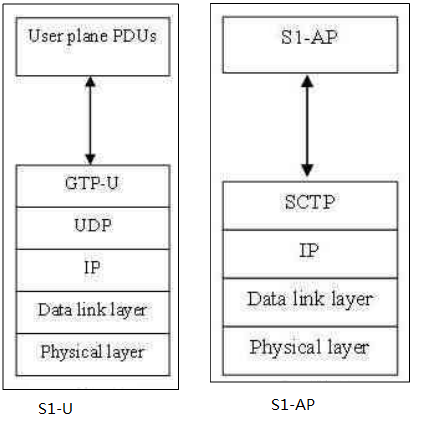
\includegraphics[width=2in]{images/S1-U.png}
          \caption{Interface S1}
          \label{Fig.S1}
      \end{figure}

\section{Introduction des données}
%\,\up{\cite{specifi}}
Après quelque semaines de négociation avec les employés de différents départements de la CMCC, ils nous ont fourni deux versions de données, et ses spécifications du format\cite{specifi}. Nous avons trouvé que CMCC n'a pas de accès direct aux données, et le fournisseur d'équipement a modifié le spécification fournir par CMCC, et il y a des erreurs dans les données fourni par les fournisseur d'équipement.

Ils nous ont envoyé $11$ dossiers, chaque dossier correspond à un service. les services sont 'rtsp', 'dns','mail', 'ftp', 'http-wap', 'mms', 'p2p', 'realtimecom', 'VoIP' et les données de signalisation entre \textsc{e-utran} et MME 'S1AP-NAS'\ref{dossier}. 
      \begin{figure}[H]
          \centering
          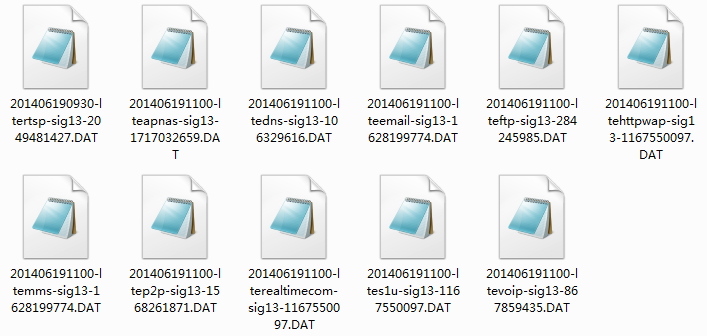
\includegraphics[width=5in]{images/data.png}
          \caption{les dossiers de données}
          \label{dossier}
      \end{figure}
Et nous avons trouvé que pour les services comme 'VoIP' et 'RTSP', ils sont très peu de données \ref{table.nombre}. Donc nous avons décidé de utiliser le donnée du service 'HTTP'.

\begin{table}[H]
\centering
	\begin{tabular}{|>{\centering\arraybackslash}p{4 cm}|>{\centering\arraybackslash}p{4 cm}|}
	\hline \textsf{L'interface }& \textsf{Nombre de ligne} \\ 
	\hline S1-AP & $240$ \\ 
	\hline RTSP &$ 35$ \\ 
	\hline DNS  & $272562$ \\ 
	\hline Maill & $44$ \\ 
	\hline FTP &$ 71$ \\ 
	\hline HTTP-WAP & $50854$ \\ 
	\hline MMS & $193$ \\ 
	\hline P2P & $515$ \\ 
	\hline Realtimecom & $2082$ \\ 
	\hline S1U &$ 89759$ \\ 
	\hline VoIP & $28$ \\ 
	\hline 
	\end{tabular} 
	\caption{les dossiers de données}
	          \label{table.nombre}
\end{table}


\subsection{Prétraitement de données}
Dans le dossier de HTTP, il y a $50854$ lignes, tous les données sont collectées par les capteurs placer entre le Service-Gateway et l'eNodeB. le capteur enregistre un ligne de donnée quand un processus est fini. chaque ligne a $76$ attributs \ref{Fig.HTTP}, qui contient des informations de UE (IMEI, IMSI, etc), les trafic de la liaison montante et la liaison descendante et le temps, la adresse IP de UE, eNodeB et S-GW, le port de UE, eNodeB et S-GW, le délai du service, le site web, cookie, et aussi le début temps et le temps d'arrêter.
les données sont collectent dans $20.92$ minutes \Ref{fig:lasttime}.
      \begin{figure}[H]
          \centering
          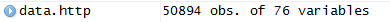
\includegraphics[width=3.5in]{images/http.png}
          \caption{les données du service HTTP}
          \label{Fig.HTTP}
      \end{figure}
      
      \begin{figure}[H]
\centering
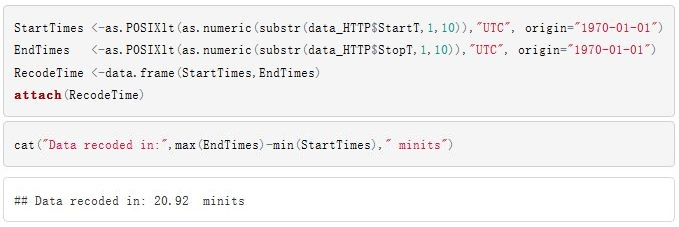
\includegraphics[width=15Cm]{images/lasttime}
\caption{Les données sont collectent dans 20.92 minutes}
\label{fig:lasttime}
\end{figure}


En analysant des données, nous avons trouvé des erreurs de données, et le fournisseur nous a confirmé que ces sont les défaut de leur système 4G. Pour les attributs 'IMSI', 'IMEI', 'MSISDN', $90$ \% de lignes sont vides, ce qui ne sont pas vides, les contenus sont illisible, et peuvent provoquant des erreurs de lecture \ref{fig:errorData}. Et nous avons trouvé que dans les contenus de certains lignes sont bizarre. 
\begin{figure}[H]
	\centering
	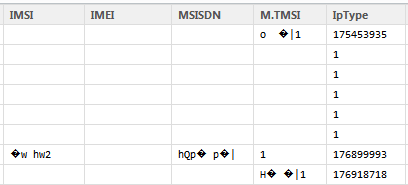
\includegraphics[width=0.7\linewidth]{images/errorData}
	\caption{erreur du codage BCD}
	\label{fig:errorData}
\end{figure}
Dans ce processus, le 'Down Link Online Time' égale à  $0$ ms , mais il a téléchargé $746$ bits, c'est clairement un erreur du données.
\begin{figure}[H]
	\centering
	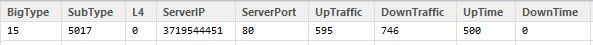
\includegraphics[width=0.9\linewidth]{images/bizarre}
	\caption{Erreur de la donnée}
	\label{fig:bizarre}
\end{figure}

 Nous avons décidé de ne utiliser les données avec ce type de erreur, à la fin, en supprimant ses données, il nous reste $37865$ lignes ($50894$ lignes en origine, $13029$ lignes ont été supprimé)  \ref{fig:newdata}.
 
\begin{figure}[H]
	\centering
	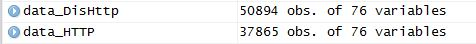
\includegraphics[width=0.8\linewidth]{images/newdata}
	\caption{Prétraitement des données}
	\label{fig:newdata}
\end{figure}

Dans certains lignes, il y a des erreurs de décompte. par exemple, dans un processus, il a téléchargé  $17$ paquets IP, et il a  $7448$  paquets sont désordre, et  ré-téléchargé  $6384$ paquets  \ref{fig:défaut}. Les données ne sont pas correct, donc nous ne pouvons pas utiliser ses donnée pour calculer les délai du service HTTP.  
\begin{figure}[H]
	\centering
	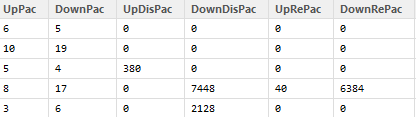
\includegraphics[width=0.7\linewidth]{images/11}
	\caption{Défaut de la système}
	\label{fig:défaut}
\end{figure}

\section{Solution existant}     
L'optimisation du service téléphonie est très important. L'opérateur a construit un immense réseau télécommunication, mais a cause de la mauvaise configuration du système, les utilisateur ne sont pas satisfais avec les services, les investissement n'a pas été remis. Donc les entreprises comme IBM, Huawei, et l'autre fournisseur du équipement essaient de trouver la meilleure solution. 

Maintenant, nous pouvons trouver beaucoup de papier sur l'optimisation du réseau télécommunication, mais les articles sont basé sur réseau 3G ou 2G, et la technique qu'ils utilisent ne sont pas convainquent. 

La technique utilise le plus souvent s'appelle 'KQI' ( Key Quality Indicator) \ref{fig:kqi}, cette méthode a été beaucoup utilisé. Et cette technique peut généralement divisé en deux étapes. d'abord, nous devons calculer le score de KPI, pour calcule le KPI en premier, il faut analyser le processus d'un service et choisir les indicateur de performances. Ensuite, nous pouvons calculer le score d'un processus en utilisant un équation linéaire, le poids de chaque attributs change selon le service, par exemple, pour le service SMS, le délai porte peu de l'importance, mais le délai du service est important pour le service HTTP. \textsf{à} la fin, nous pouvons calculer le KQI à avec les KPI \cite{kqi}. Mais les poids sont défini par les experts, et les valeurs peut-être fausse ou pas précis. Et par fois le score est bonne mais l'expérience de l'utilisateur n'est pas bon.
\begin{figure}[H]
\centering
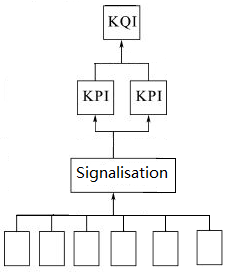
\includegraphics[width=5cm]{images/kqi}
\caption{KQI}
\label{fig:kqi}
\end{figure}

KPI est un des indicateurs de qualité axés sur les performances du réseau, mais il ne reflète pas directement l'expérience de la qualité de service de l'utilisateur, parce que les expériences de l'utilisateur sont difficile à mesure. Donc la technique QoE a été inventé. QoE défini la performance, de la qualité de service et l'expérience de l'utilisateur de l'ensemble du réseau à partir de l'utilisateur.

Les utilisateurs ont nombreuses exigences pour les services téléphonie, ils peuvent être résumées comme deux aspects: la fiabilité et le confort. La fiabilité fait référence à l'activité de l'accessibilité, la disponibilité et la durabilité. Le confort est une qualité de service, est un indice de la perception directe de l'utilisateur, qui dépend à l'expérience de l'utilisateur \cite{QoE}. Les relations entre QoE et QoS KPI sont: la fiabilité du service \ref{table.fiabilité}, le confort du service \ref{table.confort}. Maintenant, la technique de QoE a été beaucoup utilisé pour le service vocaux. Et a cause de la complexité des services de données, il n'y a pas un standard de QoE pour les services de données. 

\begin{table}[H]
	\centering
	\caption{Fiabilité du service }
	\label{table.fiabilité}
\begin{tabular}{|c|c|}
\hline \rule[-2ex]{0pt}{5.5ex} KQI & QoE \\ 
\hline \rule[-2ex]{0pt}{5.5ex} Accessibilité & Taux de succès  \\ 
\hline \rule[-2ex]{0pt}{5.5ex} Disponibilité  & Temps d'accès aux services \\ 
\hline \rule[-2ex]{0pt}{5.5ex} Durabilité & La durée de l'accès des services \\ 
\hline 
\end{tabular} 
\end{table}

\begin{table}[H]
	\centering
	\caption{Confort du service}
	\label{table.confort}
\begin{tabular}{|>{\centering\arraybackslash}p{5 cm}|>{\centering\arraybackslash}p{6 cm}|}
\hline KQI & QoE \\ 
\hline  & Taux de perte de paquets de couche d'application \\ 
\hline  & Le débit moyen  \newline \\ 
\hline La qualité du service de transmission & Stabilité de la transmission \\ 
\hline & Le bout en bout délai moyen \newline  \\ 
\hline & Gigue \newline  \\ 
\hline Le persistant de la connexion de service & La vitesse et la difficulté du service d'assistance\\ 
\hline 
\end{tabular} 
\end{table}

En utilisant la technique KQI et QoE, nous peuvent mesurer la qualité des différents services, les résultats peuvent aider les opérateurs trouver les services de mauvaise qualité, les opérateur peuvent améliorer les services selon le résultat, finalement améliorer la notation de l'utilisateur.  

Le résultat de KQI dépend seulement aux performances du réseau, donc nous avons besoin les informations des performances de réseau. Et la technologie QoE besoin Le résultat de KQI et les feed-back de l'utilisateur, le feed-back peut obtenir par l'enquête ou les plaintes des utilisateurs,  et par les mesures directs.

Aussi il y a un groupe qui utilise le comportement de l'utilisateur pour défini la qualité du service\cite{UB}. Le groupe utilise cette méthode dans le service vocaux, il cherche le situation comme l'utilisateur accroche et ré-appel le même personne. \textsc{à} la fin, cette méthode aide l'opérateur corriger le paramètre d'erreur.

Selon l'article le cette méthode peut aider l'opérateur trouver les défaut du système, mais il aa nombreuses restrictions, par exemple, nous ne pouvons pas utiliser cette technologie dans le service de SMS, etc.

\subsection{Notre solution}

La méthode qui utilise le comportement de l'utilisateur est intéressant, mais nous trouvons qu'elle peut utiliser seulement dans le service vocaux, nous n'avons pas trouvé les règles similaire dans l'autre service. D'ailleurs, le réseau LTE ne support pas le service vocaux, donc il n'existe pas optimisation du service vocaux dans réseau LTE et nous n'avons pas de données.

La technique QoE est bien aussi, mais d'abord, nous avons besoin les réponses des utilisateurs, mais nous n'avons pas assez de temps, et des raisons financières, CMCC ne peut pas nous fournir ces données. Et le équation qu'on utilise pour calcule KPI ne sont pas convaincante, voici un exemple d'un équation pour calcule la disponibilité du réseau\ref{fig:kpi}. 
\begin{figure}[H]
\centering
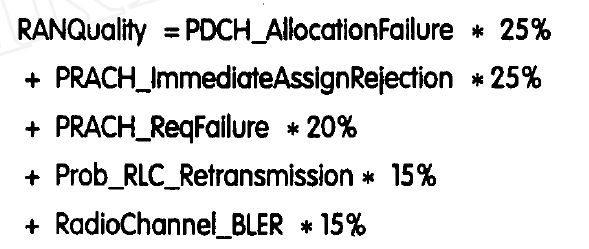
\includegraphics[width=0.7\linewidth]{images/kpi}
\caption{Un example de équation pour calculer la disponibilité}
\label{fig:kpi}
\end{figure}


q





















